\graphicspath{{img/results}{img/results/out}}

\chapter{Results}
\label{ch:results}
This chapter will present the results of the smarticle experiments in the TASEP. We will start by setting a baseline with the classical TASEP and analyze how different speed distributions affect this purely stochastic system. Next, we will compare the results with a simple hard-coded policy, before moving on to the smarticle training. We will analyze the results of the smarticle training for different reward structures and compare them to the baseline. 

\section{Notes on measuring time and current}
\label{sec:time_current}
The classical TASEP is defined for continuous time. Each particle moves according to its own internal clock. In the numerical version treated in this thesis, time has to be discretized. The discrete time step should be defined in a way that allows time averages of observables in the discrete version and the continuous version to coincide. We base our time step definition on the fact that in the continuous version, the \textit{average} number of jump attempts per second is constant. We therefore define our time step as a fixed number of \textit{update attempts}. An update attempt is the picking of a random grid cell and the attempt to move the particle in that cell, \textit{if it is occupied}. This means that also in the discrete version, the number of \textit{jump attempts} per second is constant in the time average, while it can fluctuate over short time scales.
\\
\\
In this thesis, the time step is specifically defined as \textit{one} update attempt. This makes it easy to define a particle \textit{current}, which is independent of the system size. The current is defined as the number of actual forward jumps per \textit{update attempt}. This of course has the dimension of a particle current \textit{density}, but it is still called \textit{current} in the lattice gas literature. It is the more useful quantity to work with, as it makes it easy to compare different systems. 
\\
\\
Note that this definition of the time step differs from the prevalent definition of the Monte Carlo time step in the literature \cite[ch. 3.2]{daquila_monte_nodate}, where one time step is defined more naturally as one Monte Carlo sweep. A Monte Carlo sweep is defined as $N$ update attempts, where $N$ is the number of particles in the system. 

\newpage

\section{Setting a Baseline: Classical TASEP}
\label{sec:baseline}
\begin{wrapfigure}{R}{0.45\textwidth}
    \raisebox{0pt}[\dimexpr\height-0.6\baselineskip\relax]{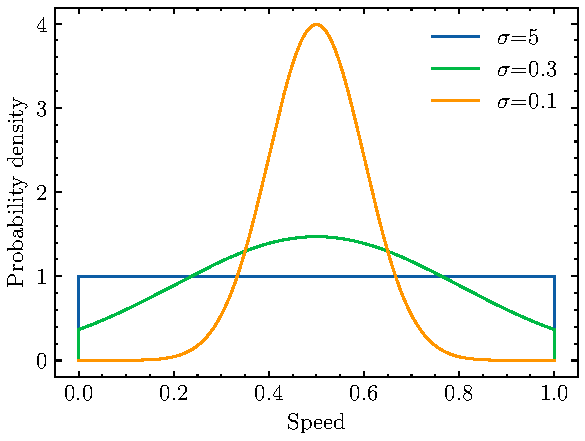
\includegraphics{truncated_normal.pdf}}
    \caption{Normalized truncated normal distributions with mean $\mu=0.5$ and different standard deviations $\sigma$.}
    \label{fig:speed_dists}
\end{wrapfigure}
This section will use the classical 2D (T)ASEP as introduced in section \ref{sec:2d-tasep}. We will make it totally asymmetric in the horizontal direction (the \textit{forward} direction) by setting the probability $p$ to jump forward to $1/2$ and the probability $q$ to jump backward to $0$. The vertical direction (the \textit{up/down} direction) will be symmetric with probabilities $a=b=1/4$. The system has periodic boundary conditions in both directions. We will analyze a $128 \times 32$ system and a narrower $128 \times 6$ system. Both systems will be initialized with a checkerboard pattern of particles and holes, yielding a density of $\rho = 1/2$. This density will be chosen for most experiments, as it is dense enough for the different policies and speed distributions to have a significant effect on the system, but not so dense that the system is always jammed. Speeds will be drawn from a truncated normal distribution with mean $0.5$ and different standard deviations $\sigma$. The distribution is truncated at $0$ and $1$, so that speeds are always in that range. Two example speed distributions are shown in figure \ref{fig:speed_dists}. 

\subsection{Finding the Steady State}

When we want to compare the average current of different ASEP configurations, we have to make sure that the system has reached a steady state. The steady state has been reached when the current fluctuates around a constant mean value without an overall upwards or downwards trend. The time it takes to reach the steady state depends on the system size, the density and the initial conditions. When using a checkerboard setup for example, it's intuitive that the current will be very high in the beginning of the simulation, as every particle has an empty site in front of it and can move forward. As time passes, the probability of being able to move forward decreases (for different reasons that we will examine in the next paragraphs), and the mean current drops, asymptotically approaching the steady state current.
\\
\\
Figures \ref{fig:currents_fixed_sigma_128x32} and \ref{fig:currents_fixed_sigma_128x3} show the current as a function of time steps since initialization of the system to the checkerboard pattern for different speed distribution standard deviations $\sigma$. We can see that for small $\sigma$, when all particles have similar speeds, the current converges quickly and reaches a steady state after about 100,000-150,000 time steps. For larger $\sigma$, particles have different speeds and the equilibration phase takes longer, as jams form and dissolve and slow particles move very rarely. For $\sigma = 5$, especially in the narrow system (Fig. \ref{fig:currents_fixed_sigma_128x3}), we see that the steady state is still not quite reached after 300,000 time steps. 
\\
\\
One could expect the equilibration time to be roughly proportional to the number of Monte Carlo sweeps that have passed. This however is not the case, as we can see by comparing figures \ref{fig:currents_fixed_sigma_128x32} and \ref{fig:currents_fixed_sigma_128x3}. The narrow system has almost 11 times fewer particles than the wide system and thus performs about 11 times more Monte Carlo sweeps in the same number of time steps. However, the equilibration time is not 11 times shorter, but seems to be about the same, or even longer. We can conclude that the number of time steps is a better measure of the equilibration time than the number of Monte Carlo sweeps.
\\
\\
For the following experiments, the steady state current will be calculated by running the simulation for 600,000 time steps and averaging the current over the last 150,000 time steps. This ensures that the system has reached a steady state even for the configurations that take longer to equilibrate.
\\
\begin{figure}[H]
    \centering
    \begin{subfigure}{\textwidth}
        \centering
        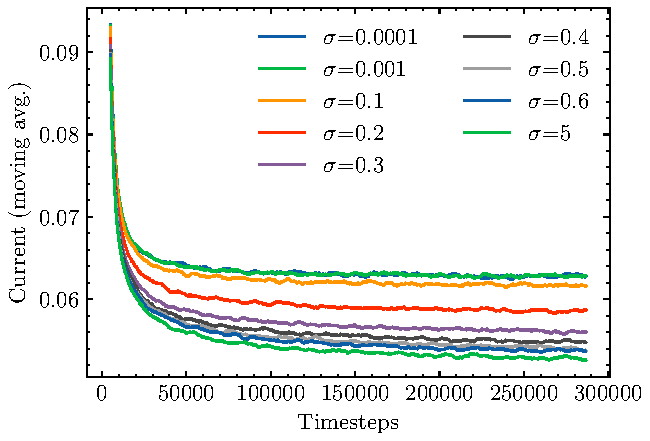
\includegraphics{currents_fixed_sigma_128x32}
        \caption{System size: 128x32}
        \label{fig:currents_fixed_sigma_128x32}
    \end{subfigure}
    \par\vspace{1cm}
    \begin{subfigure}{\textwidth}
        \centering
        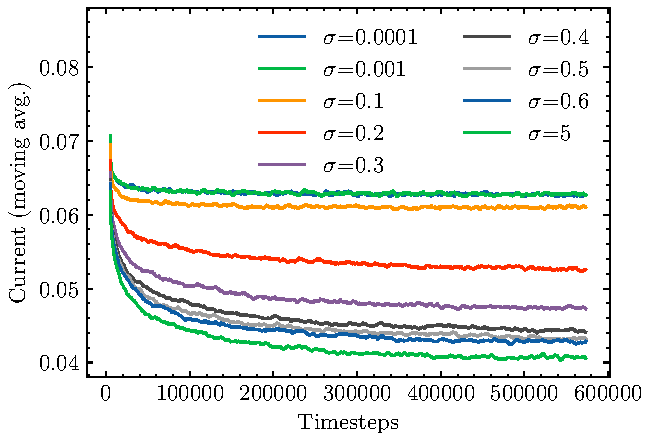
\includegraphics{currents_fixed_sigma_128x3}
        \caption{System size: 128x3}
        \label{fig:currents_fixed_sigma_128x3}
    \end{subfigure}
    \caption{Current as a function of time steps since initialization of the system to the checkerboard pattern for different speed distribution standard deviations $\sigma$ and two different system sizes. The data is averaged over 800 independent runs and plotted with a moving average over 5000 time steps.}
\end{figure}


\section{Steady State Current as a Function of System Size and Speed Distribution}
\label{sec:steady_state_current}
Now that we have established a definition of what is to be measured and how this measurement can be done from the simulation data, we can check if the measured steady state current is in accord with our intuition and how it depends on the system parameters. 

\subsection{Theoretical Expectation}
\label{sec:theoretical_expectations}
In order to derive an expression for the expected value of the current, we closely examine what happens during one time step. This will help us to understand the probability of an actual forward move happening during one time step, which, by our definition, is the current.
\\
The following steps are performed during one time step:
\begin{enumerate}
    \item Pick a random grid cell.
    \item If the cell is occupied (probability $p_{occ}=\rho=0.5$), perform a move attempt as follows:
    \item Check the speed: The move attempt is continued with probability $p_{spd}=\text{speed}$.
    \item If the move attempt is continued, pick a direction (forward has probability $p=1/2$).
    \item If the target cell is empty (probability $p_{emp}\approx 1-\rho$), perform the move.
\end{enumerate}
Where the expression $p_{emp}\approx 1-\rho$ only holds for an approximately uniform density distribution throughout the system. The average speed $\bar{v} = /bar{p_{spd}}$ is the expectation value $\mu$ of the speed distribution, which is set to $0.5$ in all experiments. The total probability of a forward move in one time step is the product of the probabilities of the individual steps:
\begin{align}
    \langle J\rangle &\coloneqq p_{occ} \cdot p_{spd} \cdot p \cdot p_{emp} \label{eq:current_theory} \\
                     &\approx p \cdot \mu \cdot \rho (1-\rho) = \left(\frac{1}{2}\right)^4 \nonumber \\
                     &= 0.0625 \text{.}\nonumber
\end{align}
More thorough derivations of this expression for ASEP systems with equal speeds can be found in the literature, for example in \cite[section 2.3.2]{daquila_monte_nodate}. Equation \ref{eq:current_theory} also confirms that our choice of the density $\rho=1/2$ is optimal for maximizing the current in the system, as the maximum of the function $f(\rho) = \rho(1-\rho)$ is at $\rho=1/2$.


\subsection{Results of the Simulation}
\label{sec:results_simulation_current_sigma_size}
Figure \ref{fig:steady_state_current_sizes_log} shows the steady state current as a function of the speed distribution's standard deviation $\sigma$ for different system sizes. The steady state current has been obtained as explained previously and the data is averaged over 800 independent runs. For all system sizes, we observe a constant maximum current for $\sigma \ll 1$ that is only very slightly above the expected value of $0.0625$. The slight increase is probably due to the fact that the steady state is only reached in the limit of infinite time. Although being very close, after 450,000 time steps, the current is still dropping a tiny amount, as can be seen in figure \ref{fig:currents_fixed_sigma_128x3}. 
\\
As the width of the speed distribution grows to values of $\sigma \approx 1$, the current drops quickly before asymptotically converging to the minimum value, following a horizontally inverted logistic function. The logistic curve's midpoint is at $\sigma_0 \approx 0.2$ and the width of the transition is $\Delta \sigma \approx 1$. This makes sense, as the speed distribution is truncated at $0$ and $1$, so for values of $\sigma$ close to $0$, all particles have speeds close to $0.5$ and the current is close to its maximum value. When $\sigma$ grows, the speeds in the system get more and more diverse, until $\sigma$ reaches $1$, where the speed distribution is almost uniform and doesn't change much anymore. 
\\
The current drops although the mean speed in the system is still the same, because the probability of a particle moving forward is not only dependent on its own speed, but also indirectly on the speeds of the particles in front of it. The slow particles bottleneck the current as the fast particles have to wait for them to move forward, creating a jam. This effect is more pronounced in narrower systems, as small jams block a higher proportion of the system. In wide systems, particles can avoid jams by moving around them, and even if there's a jam in almost every lane, the probability of these jams to all be in the same column is very low. In narrow systems, this can happen, forming a wall of slow particles, which is hard to penetrate. This is clearly visible in figure \ref{fig:steady_state_current_sizes_log}, where the total drop in current is much higher for narrow systems. 
\\
\\
Looking back at equation \ref{eq:current_theory}, we can also try to explain this behavior theoretically. When jams form, the density in the system is not uniform anymore. Instead, there are regions of high density (jams) and regions of low density (empty lanes). This increases the mean density in the neighborhood of a random particle, decreasing $p_{emp}=(1-\rho)$ and thus the probability of a forward move.  

\begin{figure}[H]
    \centering
    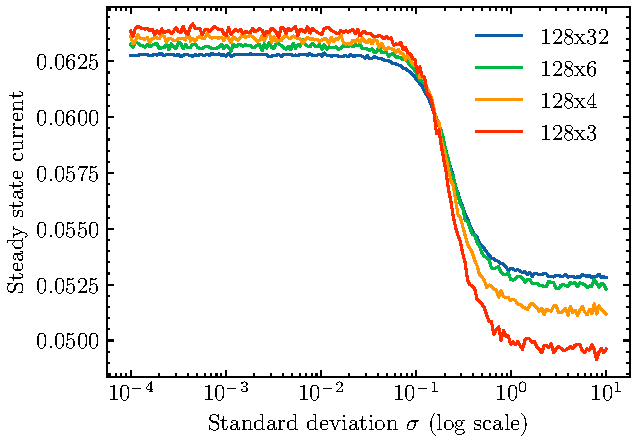
\includegraphics{steady_state_current_sizes_log.pdf}
    \caption{Steady state current as a function of the speed distribution's standard deviation $\sigma$ for different system sizes. Steady state current is calculated as the average current over all remaining time steps after the steady state has been reached (the current has stopped dropping). The data is averaged over 800 independent runs.}
    \label{fig:steady_state_current_sizes_log}
\end{figure}

\section{A Naive Policy}
We have now established a baseline current for different system sizes and speed distributions. Before we move on to the smarticle training to try to optimize the current with reinforcement learning, let's see if we can improve the current with a simple hard-coded policy. 
\\
One of the simplest and yet effective policies is to always move forward if possible. Especially when we choose $\sigma$ to be very small and all particles have similar speeds, this policy should be very effective, as it keeps the density uniform and avoids jams. Furthermore, it is very easy to implement without writing any new code by just setting the probability $p$ to move forward to $1$ and all other probabilities ($a,b,q$) to $0$.
\\
\\
Figure \ref{fig:steady_state_current_always_forward} compares the steady state current of this policy with the current from the last experiment, again as a function of the width of the truncated normal distribution. We can see that for small $\sigma$, our policy drastically improves the current, approximately doubling it. For larger $\sigma$, the current drops as before and drops even further, resulting in only about half the current of the baseline for $\sigma\gg 1$. 
\\
\\
The reason for the extreme drop in current is that the policy is not able to deal with jams at all. The current in each lane is limited to the speed of the slowest particle in that lane. The resulting measured current then is the average of the currents in all lanes. 
\\
\begin{figure}[H]
    \centering
    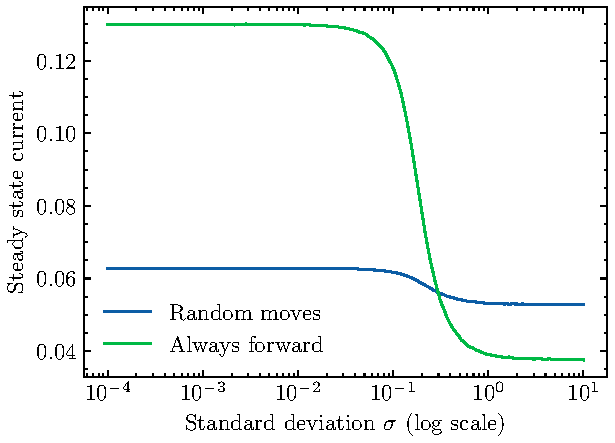
\includegraphics{steady_state_current_both_log.pdf}
    \caption{Steady state current as a function of the speed distribution's standard deviation $\sigma$ for two different ASEP configurations. \enquote{Random moves} has a probability of $p=1/2$ to move forward probabilities $a=b=1/4$ to move up/down. \enquote{Always forward} has $p=1$ and $a=b=0$. A system of size 128x32 was used. The data is averaged over 800 independent runs.}
    \label{fig:steady_state_current_always_forward}
\end{figure}
The current achieved by this policy for small $\sigma$ is even more interesting. It can be used as a new, very strong baseline for the smarticle training in systems with equal speeds. At first glance, it might even seem like the theoretical maximum current. Finding this maximum analytically is not trivial and goes beyond the scope of this thesis. However, we can try to find an upper bound for the current by looking at equation \ref{eq:current_theory} again:
\begin{align*}
    \max(\langle J\rangle) &= \max(p_{occ} \cdot p_{spd} \cdot p \cdot p_{emp}) \\
                           &\le \max(p_{occ}) \cdot \max(p_{spd}) \cdot \max(p) \cdot \max(p_{emp}) \\
                           &= \rho \cdot \mu \cdot 1 \cdot \max(p_{emp}) \\
                            &= 0.25 \cdot \max(p_{emp})\text{,}
\end{align*}
where $\max(x)$ is the maximum expected value of $x$ at a random time step, for a randomly picked particle. It therefore represents the maximum time-averaged value of $x$ that can be achieved by any policy. I have set $p_{occ}=\rho$, $p_{spd}=\mu$, as they are external parameters that cannot be optimized by a policy. The policy cannot influence which particle is picked at a given time step, so it cannot influence $p_{occ}$. The \textit{average} speed of a random particle will also always be the mean speed $\mu$. The maximum of $p$ that any policy can have is obviously $1$ (in general, this will not be a probability when using a policy, but the decision will be based on the particle's observation, but the maximum fraction of forward decisions is still 1). 
\\
The last factor, $max(p_{emp})$, is the hardest to approximate. There are configurations where $p_{emp}$ reaches its maximum value of $1$, but these configurations cannot last longer than one time step. In the checkerboard configuration for example, every particle has an empty site in front of it, so $p_{emp}=1$. However, as soon as one particle moves forward, two particles are immediately next to each other and $p_{emp}$ decreases. We therefore know that $\max(p_{emp})<1$.
\\
On the other hand, we know that $\max(p_{emp})\ge0.5=(1-\rho)$, as this upper bound is reached by the \enquote{always forward} policy. This places the upper bound for the current at
\begin{equation}
    0.25 > \max(\langle J\rangle) \ge 0.25 \cdot (1-\rho) = 0.125 \text{.}
\end{equation}
In order to keep $p_{emp}$ above $1-\rho$, which it would be for a randomized configuration, a policy has to intelligently fight against the disorder inevitably introduced by the random picking of particles. This is especially hard for systems with equal speeds, as the density in these systems has to be kept uniform, while also moving forward as often as possible.
\\
In the regime of high $\sigma$, where the \enquote{always forward} policy performs very poorly, $p_{emp}$ becomes a very interesting point of attack for a current-optimizing policy. When particles have very different speeds, a policy can organize the system in a way that slow particles are more densely packed than fast particles, increasing $p_{emp}$ for the fast particles while decreasing it for the slow particles. This increases the net current, as the fast particles can fulfill their potential to move forward more often. We will investigate this in more detail in the next sections.


\section{Smarticles for Current Optimization}
\label{sec:smarticle_current_optimization}
This section will present the results of different smarticle trainings for slightly different goals. The main goal is always to maximize the current, but we will different approaches to achieve this goal, utilizing many of the features of the python package introduced in section \ref{sec:implementation-smarttasep}. Although the deep Q-learning algorithm is not deterministic e.g. due to the random initialization of the neural network weights, the results presented here have shown to be reproducible. Appendix \ref{app:code} contains the code that is needed to reproduce the results with the smart TASEP python package.

\subsection{First Training: Equal Speeds}
As a first experiment, we will try to maximize the current in a system with equal speeds. We will use a system of size $128 \times 24$ and a speed distribution with $\sigma=10^{-4}$. The reward structure for this first experiment is very simple and includes only the \texttt{social\_reward} in addition to the default reward. Optimal hyperparameters for this reward structure have already been found in section \ref{sec:hyperparam_optim}. The training was run for 500,000 time steps, with a reset of the environment after every 100,000 time steps.
\\
\\
Figure \ref{fig:first_training_screenshot} shows a screenshot of the real-time visualization of the training after $\approx 350,000$ time steps. We can see that the training is almost converged at this point, confirming that $500,000$ time steps are enough to reach convergence for this problem. After the training, the simulation was run with a greedy policy for another $1.5$ million time steps to measure the steady state current. The results are shown in figure \ref{fig:equal_speeds}. 
\\
We can see that the steady state is reached fairly quickly compared to the stochastic policies. The current fluctuates around a mean value of $0.152$, which is about 143\% higher than the baseline (0.0625) and about 22\% higher than the \enquote{always forward} policy (0.125). The amplitude of the fluctuations is about $0.03$, which is about 20\% of the mean value, but the lowest current measured is still higher than the \enquote{always forward} policy's current. 
\\
\\
These first results are already very promising. One would expect the \enquote{always forward} policy to already perform very well in this simple environment, but the smarticles are able to outperform it by a significant margin. This can be seen as a clear proof of concept, which motivates further experiments with more complex reward structures and speed distributions, as will be presented in the next sections.
\begin{figure}[H]
    \centering
    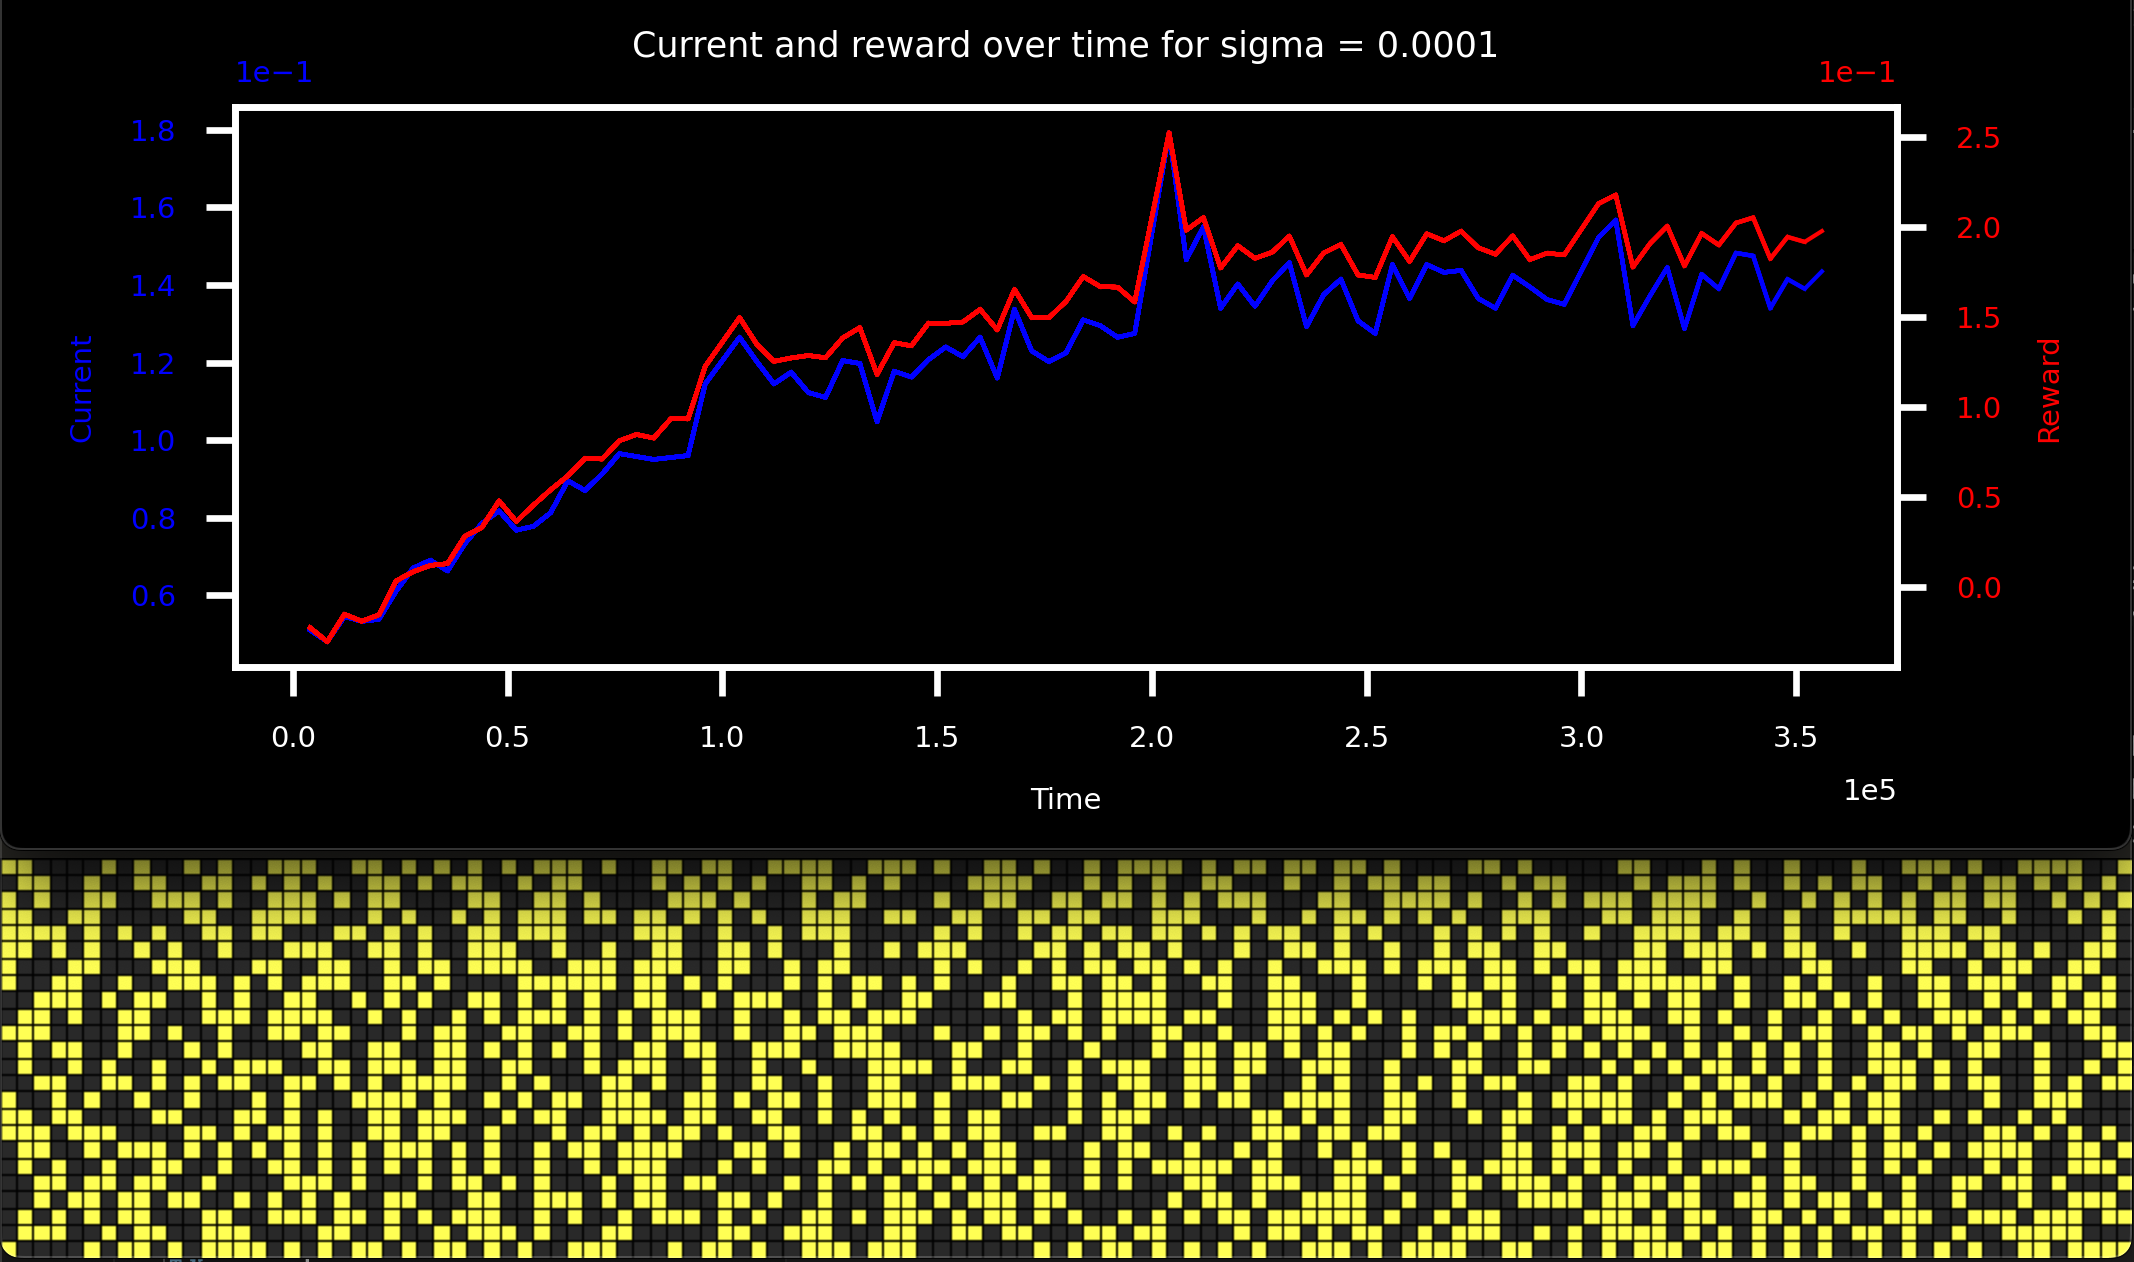
\includegraphics[width=\textwidth]{first_training_screenshot.png}
    \caption{A screenshot of the real-time visualization of the first training, taken after $\approx 350,000$ time steps. All particles have the same speed of $0.5$, which can also be seen from their yellow color. We can see that the algorithm has almost converged at this point.}
    \label{fig:first_training_screenshot}
\end{figure}

\begin{figure}[H]
    \centering
    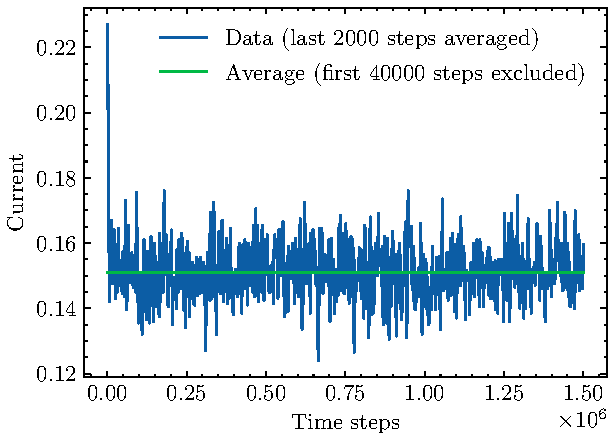
\includegraphics{equal_speeds.pdf}
    \caption{Steady state current as a function of the simulation time for the first trained smarticle agent. The green line shows the average current, which is at about $0.152$, outperforming not just the baseline by about 143\%, but also the \enquote{always forward} policy by about 22\%.}
    \label{fig:equal_speeds}
\end{figure}

\subsection{Second Training: Uniformly Distributed Speeds, Simple Reward}
\label{sec:second_training}
We will now move on to a more complex system with almost uniformly distributed speeds ($\sigma=10$). All other parameters are the same as in the first training. A screenshot during the training is shown in figure \ref{fig:second_training_screenshot} and confirms that 500,000 time steps are enough to reach convergence for this problem as well. The new agent was also tested with a greedy policy for another $1.5$ million time steps and the results are shown in figure \ref{fig:uniform_speeds}. This time, more time steps are required to reach the steady state, which makes sense, as the slow particles require more move attempts until they actually move. The mean current is at about $0.117$, again outperforming the baseline ($\approx 0.052$), this time by about 125\%. 
\\
\\
Watching the simulation, we can see that the agent has learned a policy that focuses on the small scale. No large scale structures like lanes or clusters can be observed. Instead, the global behavior is best described as a meandering flow or a trickle. The slow particles form a quasi-static maze, which the fast particles can navigate through. If the direction of movement was turned from horizontal to vertical, the trickling behavior would look like a Galton board (without the throttle on top and with periodic boundary conditions). A short video example is available at TODO.

\begin{figure}[h]
    \centering
    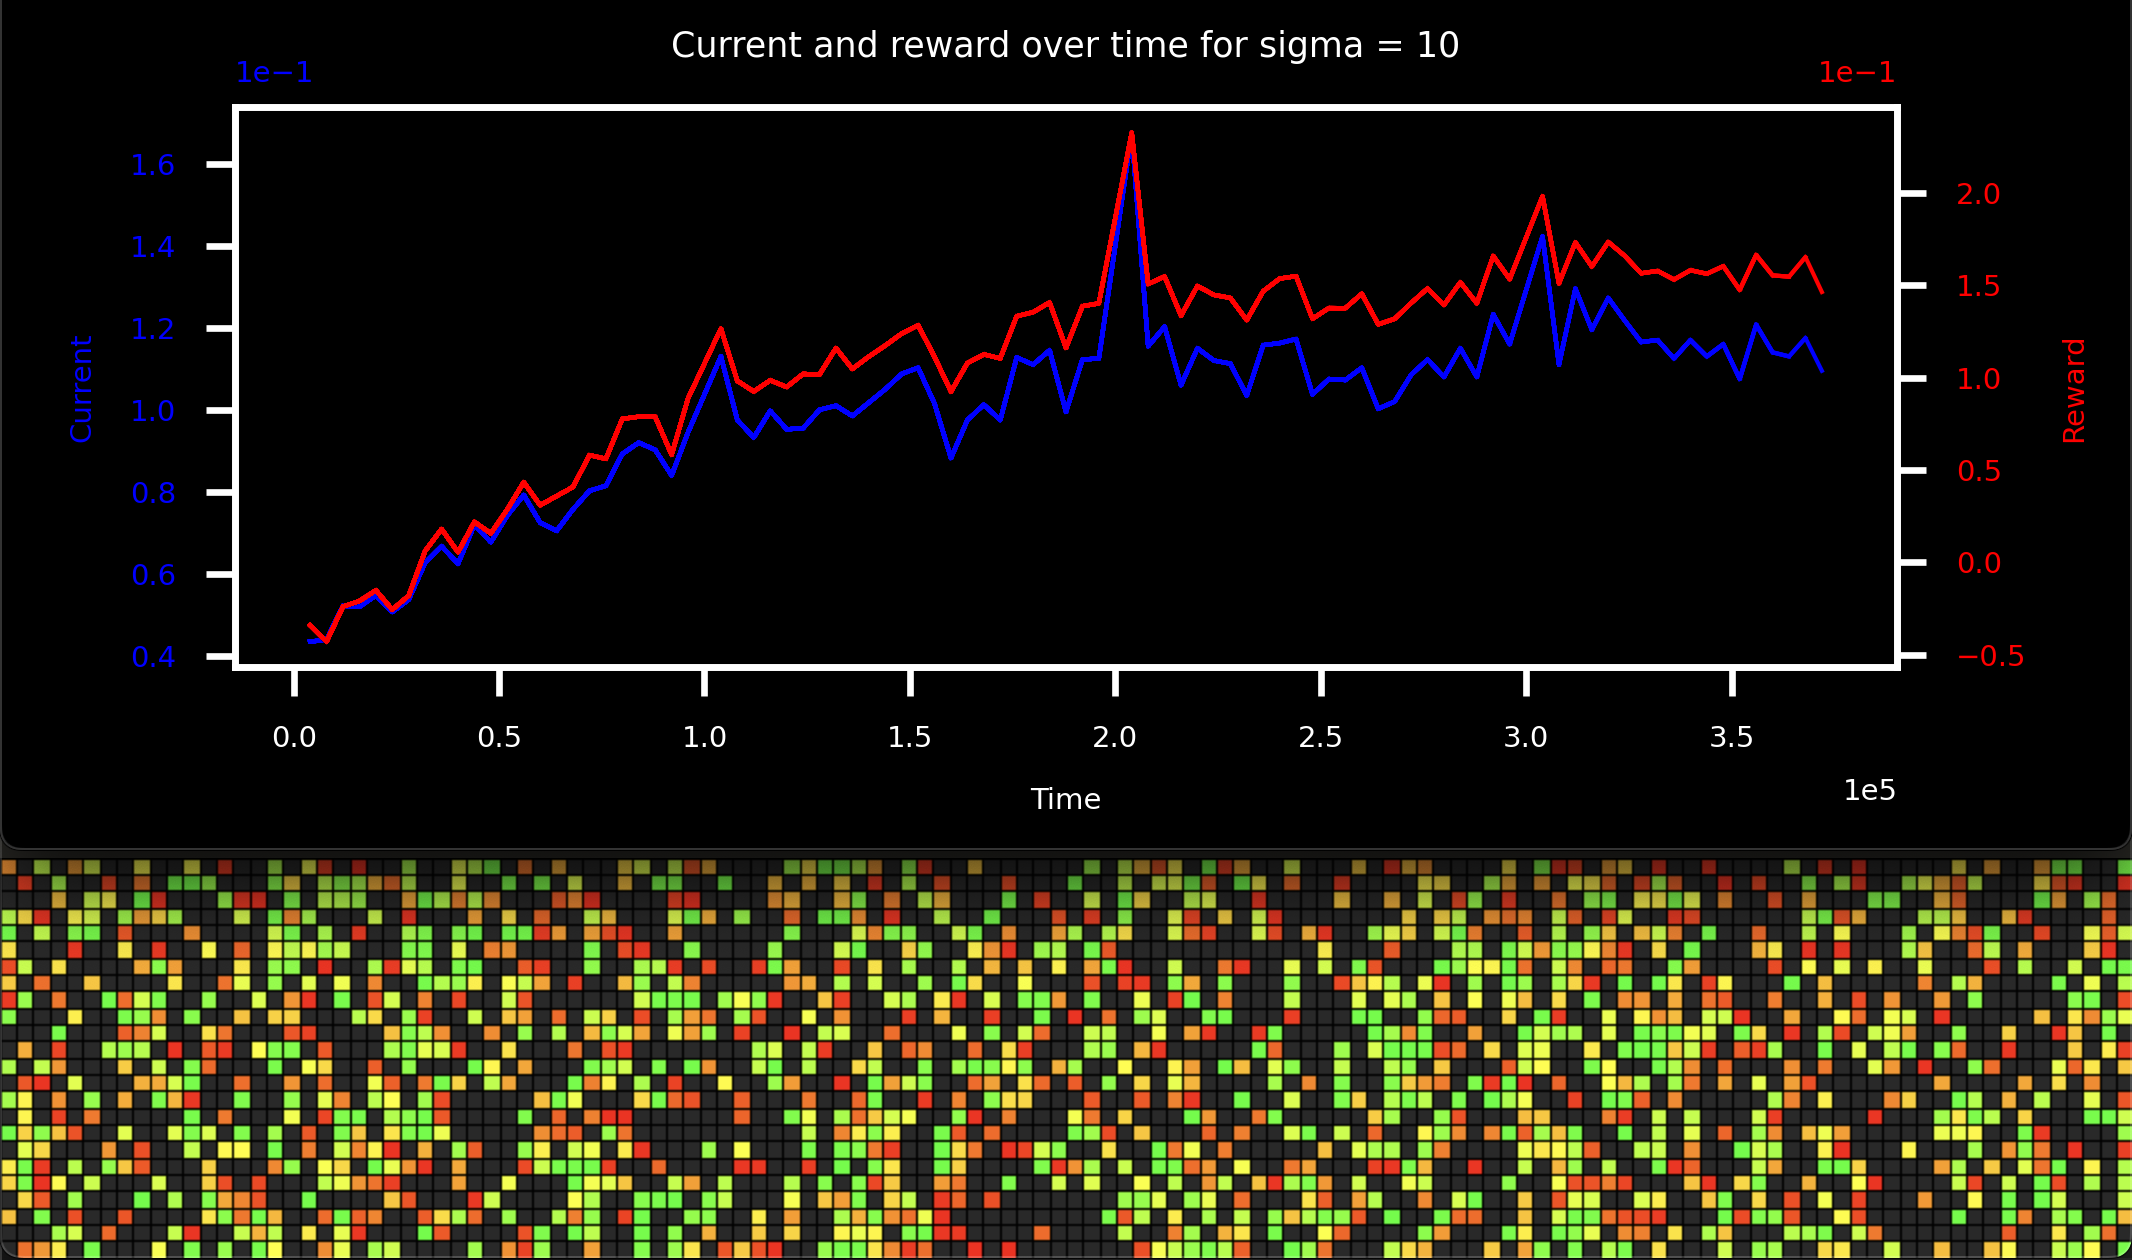
\includegraphics[width=\textwidth]{second_training_screenshot.png}
    \caption{A screenshot of the real-time visualization of the second training, taken after $\approx 350,000$ time steps. The particles have different speeds, which can be seen from their different colors. The algorithm has almost converged at this point.}
    \label{fig:second_training_screenshot}
\end{figure}

\begin{figure}[h]
    \centering
    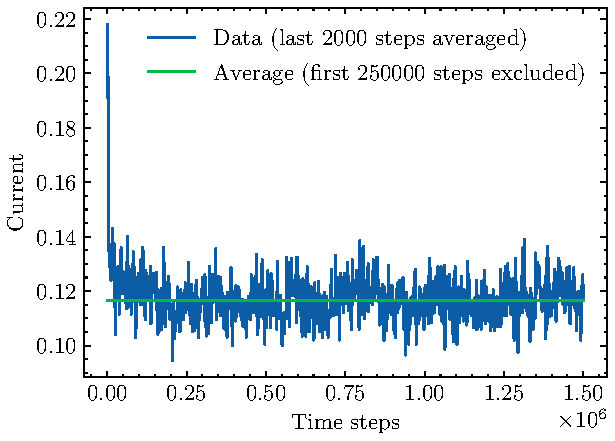
\includegraphics{uniform_speeds.pdf}
    \caption{Steady state current as a function of the simulation time for the smarticle agent trained in an environment with uniformly distributed speeds. The green line shows the average current, which is at about $0.117$, outperforming the baseline by about 125\%.}
    \label{fig:uniform_speeds}
\end{figure}

\subsection{Model Analysis: Explainability}
\label{sec:model_analysis}
We have now seen that the smarticle agent is able to outperform the baseline in two different environments. We also know the algorithm behind the training, which is used to find these optimal policies. However, we still don't know \textit{how exactly} the agent is able to achieve this performance. What is the policy that it has learned? What features of the environment are important for the agent? These questions often arise when using deep learning algorithms, as the inner workings of the neural network are not easily accessible, leading some to call deep learning a \enquote{black box} \cite{blazek_blackbox_2022}.
\\
\\
When using machine learning algorithms for real-world applications, especially in direct interaction with humans, it is important to be able to at least partially explain the decisions made by the algorithm. For this reason, a lot of research has been done in the field of \textit{explainable artificial intelligence} \cite{explainable_ai_systematic_2023}. The SHAP (SHapley Additive exPlanations) framework \cite{lundberg_unified_2017, github_shapshap_2024} for example provides a game theoretic approach to explain the output of any machine learning model. It calculates \textit{feature importance} scores, which quantify the impact of each input feature on the model's output. This can provide local explanations for individual predictions as well as global explanations for the model as a whole. Due to the limited time available for this thesis, SHAP or similar feature importance analysis methods have not yet been applied to the smarticles, but this would be an interesting topic for future research.
\\
\\
The smarticles package does however provide a simple, \enquote{hands-on} way to analyze the policies: The \texttt{Playground} class, introduced in section \ref{subsec:implementation-playground}, allows us to interactively play with the trained model. This way, we can quickly get a feeling for the policy that the model has learned. This way done for the agent trained with a uniform speed distribution. The results are shown and interpreted in figures \ref{fig:playground_1} to \ref{fig:playground_8}. 

\newcommand\newsubcap[1]{\phantomcaption%
       \caption*{\thefigure\thesubfigure: #1}}

\begin{figure}[H]
        \begin{subfigure}[T]{0.45\textwidth}
            \centering
            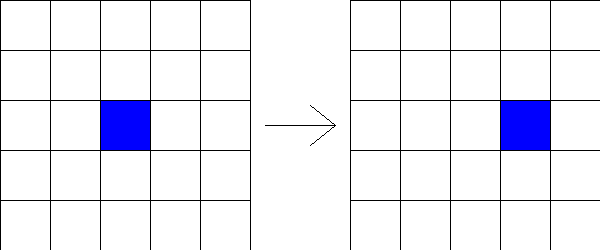
\includegraphics[width=\textwidth]{playground/1.png}
            \newsubcap{The agent knows to move forward when there is an empty site in front of it.}
            \label{fig:playground_1}    
        \end{subfigure}
        \hfill
        \begin{subfigure}[T]{0.45\textwidth}
            \centering
            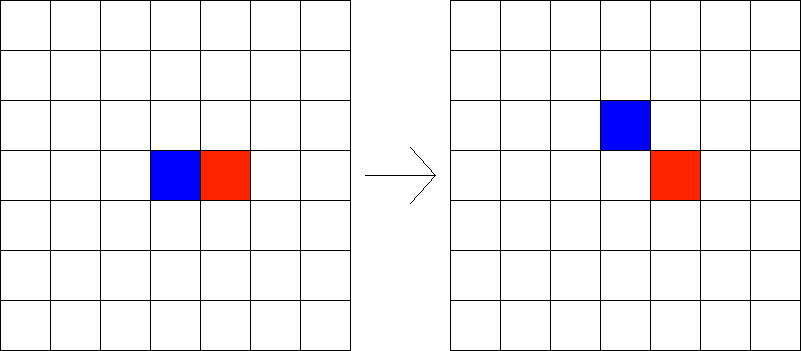
\includegraphics[width=\textwidth]{playground/2.png}
            \newsubcap{The agent knows to move around slow particles.}
            \label{fig:playground_2}
        \end{subfigure}
\end{figure}

\begin{figure}[H]\ContinuedFloat
        \begin{subfigure}[T]{0.45\textwidth}
            \centering
            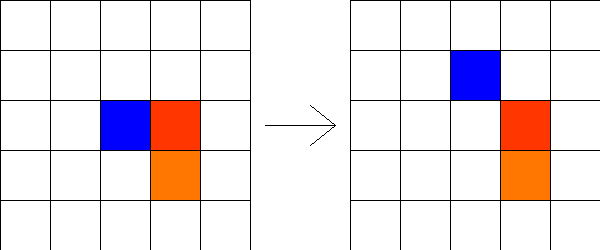
\includegraphics[width=\textwidth]{playground/3.png}
            \newsubcap{The agent knows which way around a barrier is faster. Right...}
            \label{fig:playground_3}
        \end{subfigure}
        \hfill
        \begin{subfigure}[T]{0.45\textwidth}
            \centering
            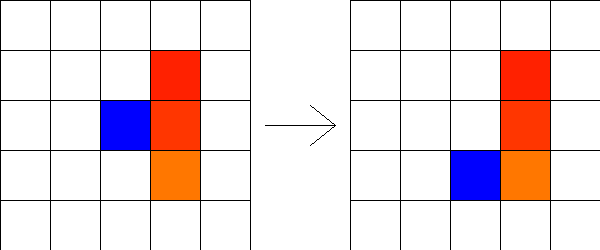
\includegraphics[width=\textwidth]{playground/4.png}
            \newsubcap{...or left.}
            \label{fig:playground_4}
        \end{subfigure}
\end{figure}

\begin{figure}[H]\ContinuedFloat
        \begin{subfigure}[T]{0.45\textwidth}
            \centering
            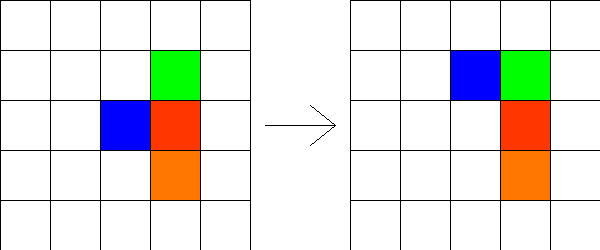
\includegraphics[width=\textwidth]{playground/5.png}
            \newsubcap{The agent knows that fast particles are more likely to move forward than slow particles.}
            \label{fig:playground_5}
        \end{subfigure}
        \hfill
        \begin{subfigure}[T]{0.45\textwidth}
            \centering
            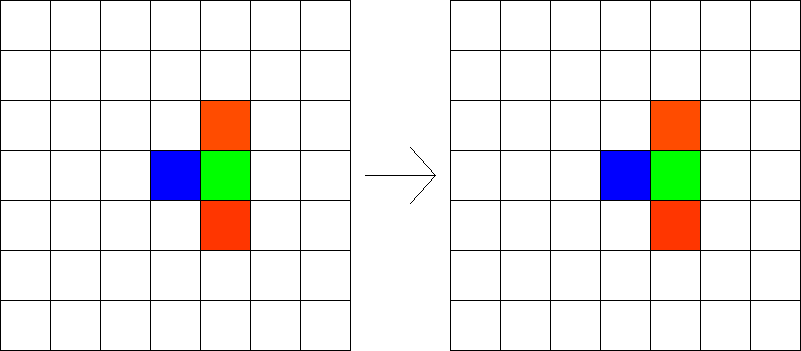
\includegraphics[width=\textwidth]{playground/6.png}
            \newsubcap{The agent knows that sometimes, it's better to wait.}
            \label{fig:playground_6}
        \end{subfigure}
\end{figure}

\begin{figure}[H]\ContinuedFloat
        \begin{subfigure}[T]{0.45\textwidth}
            \centering
            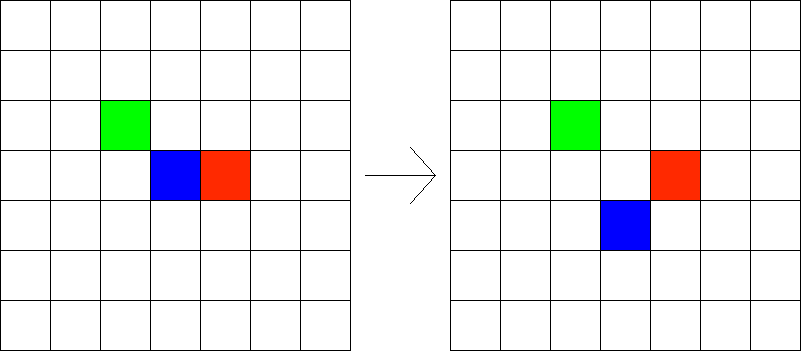
\includegraphics[width=\textwidth]{playground/7.png}
            \newsubcap{The agent tries not to block other particles, if possible.}
            \label{fig:playground_7}
        \end{subfigure}
        \hfill
        \begin{subfigure}[T]{0.45\textwidth}
            \centering
            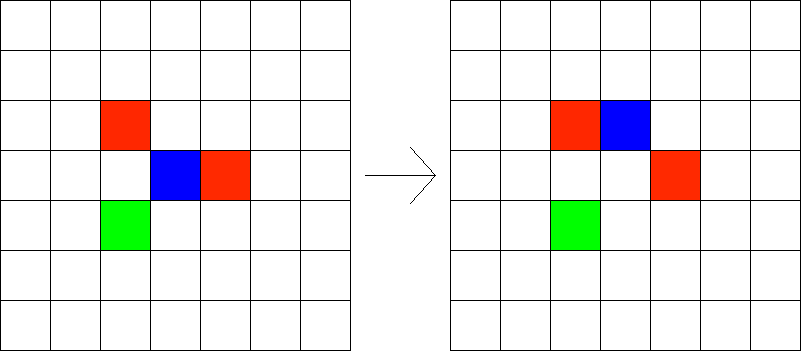
\includegraphics[width=\textwidth]{playground/8.png}
            \newsubcap{If the agent has to block other particles, it tries to block slow particles.}
            \label{fig:playground_8}
        \end{subfigure}
\end{figure}

We can see that the agent has learned a complex policy, that not only enables it to navigate around obstacles, but also takes into account the speed of the other particles that make up the obstacle. In all eight situations that were tested, the agent made the logical decision, which is also the decision that a human would make in the same situation, and it has also learned to incorporate some social behavior into its policy. A possible next step for further research on an application of the smarticles could be to dive deeper into the basic rules by which the agent makes its decisions, also quantifying the confidence of the agent in its decision. That knowledge could then be used to fine-tune the policy in areas where it is not yet optimal, to provide explainability and also to strip down the policy to a less complex, but still effective version, that uses less computational resources and is faster to evaluate. 

\section{Encouraging Global Structures}
\label{sec:global_structures}
% nice policies, but not really global structures
% when thinking of systems without periodic boundary conditions, global structures are important to keep the particles together
% also nice for different densities for different speeds, to increase the current
We have already seen two different policies that both perform very well, but until now, the smarticles have only learned to act on their own, although some social behavior is incorporated into the previous policies. It could however be beneficial to encourage the formation of global structures, like lanes or clusters. 
\\
\\
For one, this could improve the total current, as a higher priority could be assigned to the fast particles, allowing them to move in a lower density environment, while the slow particles are more densely packed. Even with uniform density throughout the system, the formation of \textit{fast lanes} and \textit{slow lanes} could be beneficial, as it prevents the fast particles from getting stuck behind slow particles.
\\
Furthermore, even outside the context of current optimization, global structures are important for the stability of the system. When the system is not periodic in the transverse direction, the particles have to be kept together to efficiently create a directed flow. Imagine a real-world application where smarticles are not moving on a tube's surface, but on a plane. In this case, the width of the particle stream would increase with the distance traveled. This is because although the mean movement in the transverse direction is zero, the variance is not. For such a system, it is important to keep the particles together, which can be achieved by encouraging the formation of global structures.

\subsection{A Physicist's Perspective on the Reward Structure}
\label{sec:physics_reward_structure}
The formation of global structures arising from microscopic interactions is an interesting point to again make the connection to physics. We can compare the way physical matter is formed from physical particles with the way that smart matter is formed from smarticles. 
\\
\\
Physical matter in thermodynamic equilibrium organizes in a way that minimizes or maximizes a certain thermodynamic potential such as the free energy or the entropy. This is the result of the microscopic interactions between the particles that make up the matter. For most systems, it is not feasible to describe the microscopic state of a system as a function of time, as the number of degrees of freedom grows exponentially with the number of particles. Instead, we use statistical mechanics to describe the system in terms of macroscopic observables, such as the density or the temperature. We can then derive the expected value of these observables by averaging over all possible microscopic states of the system.
\\
\\
Similarly, when using reinforcement learning to train a system of smarticles, we try to define a high level quantity that we want to optimize, such as the current. We then use this quantity as a reward signal to train the smarticles to maximize it. The microscopic interactions between the smarticles are learned and therefore \textit{defined} by the smarticles themselves, without us having to worry about them. In a sense, we let the smarticles discover the \enquote{physical} laws that would have to govern the system in order to maximize the reward. As a next step, we can then try to derive these laws from the trained policy, as we have done in section \ref{sec:model_analysis}.
\\
\\
Sometimes, different laws (policies) can lead to very different macroscopic behavior while still maximizing the same high level quantity. For example, the current can be maximized by a policy that keeps the system mixed, as well as by a policy that forms lanes (different local minima that the gradient descent algorithm can converge to). One could compare this to the different phases of matter in physics, where the laws that govern the microscopic interactions are the same, but the macroscopic behavior changes drastically, often also involving symmetry breaking. Here however, the laws are different, while the high level quantity that is optimized is the same. The macroscopic behavior arising from the new laws of interaction may still be very similar to the behavior arising from the old laws, but it could also be very different. 
\\
\\
When trying to encourage the formation of global structures, we are trying to nudge the smarticles towards a certain set of laws that we think will lead to the desired behavior, \textit{while still maximizing the current} (in machine learning language, we're helping the gradient descent algorithm to find a specific local minimum, instead of a random one closest to the initial conditions). We do this by incorporating a new reward signal into the reward structure, which is based on the microscopic state of the system. In order to find a suitable reward signal, we \textit{can} look back at physics, drawing inspiration from the laws that govern the formation of global structures in physical equilibrium matter.

\subsection{Global Structures - The Easy Way}
\label{sec:global_structure_easy}
The first approach that we will try is to very explicitly supply the smarticles with the structure that we want to see. This can be done by supplying the agents with their absolute position on the transverse axis (with to an arbitrary origin) as an additional input feature. We can then create a reward function that is based on this position as well as the speed of the particle. The \texttt{speed\_gradient\_reward} function in the smarticles package implements this idea. It assigns a desired lane to the particle based on its speed and then rewards the agent proportionally to the distance to that lane. The speeds are mapped to lanes using the following function:
\begin{equation}
    \Delta y=1-a\cdot\left(\frac{\left(1+a\right)}{a}\right)^{v}+a \text{,}
\end{equation}
where $\Delta y$ is the relative distance from the center ($\Delta y=1$ is a distance of \texttt{system width / 2} from the center) and $v$ is the speed of the particle. The parameter $a$ controls the steepness of the function. In the limit of $a\rightarrow\infty$, the function becomes linear, with a slope of $1$, while for small $a$, the function grows exponentially. This allows us assign a higher proportion of lanes to the fast particles. Figure \ref{fig:speed_gradient} shows the mapping for different values of $a$. The decision to put the center lane into the middle of the screen is of course arbitrary, as the system is periodic in the transverse direction. 
\begin{figure}[H]
\centering
\begin{subfigure}{\textwidth}
    \centering
    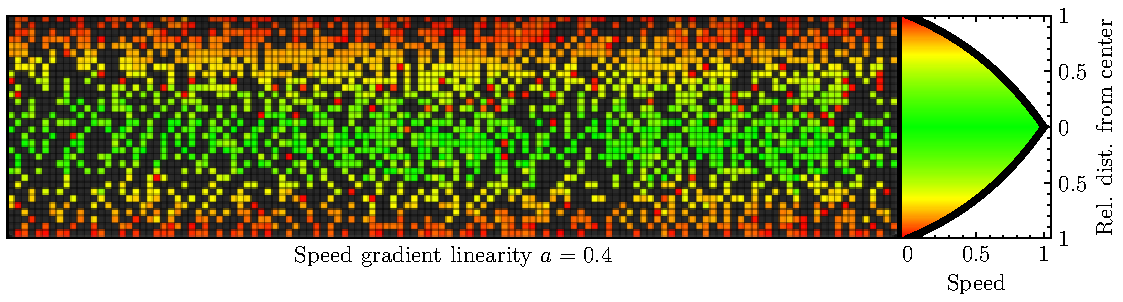
\includegraphics[width=\textwidth]{speed_gradient_0.4}
\end{subfigure}
\begin{subfigure}{\textwidth}
    \centering
    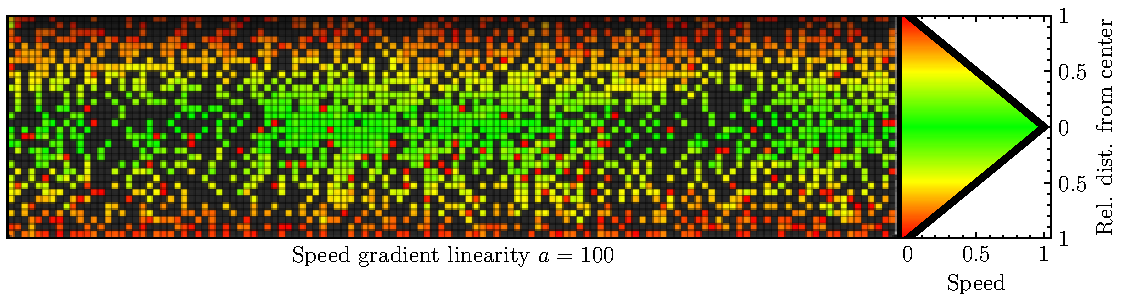
\includegraphics[width=\textwidth]{speed_gradient_100}
\end{subfigure}
\caption{The mapping of speeds to lanes in the \texttt{speed-gradient-reward} function for different values of $a$. The images left of the graph are screenshots of the real-time visualization of the simulation.}
\label{fig:speed_gradient}
\end{figure}
Figure \ref{fig:speed_gradient} also shows screenshots of the simulation after training. We can see that the formation of lanes clearly works and the actual color gradient realized by the smarticles in the system closely matches the desired gradient which is encoded in the reward. In the screenshot corresponding to a non-linear mapping ($a=0.4$), we can see that the mean density in the fast lanes is indeed lower than in the slow lanes. We will investigate the effect of this on the current in a minute. 
\\
\\
The two screenshots also include examples of imperfect behavior. For one, we always see stray slow particles in the fast lanes, as it takes them a long time to move to their desired lanes. This is something that resolves itself over time, but it also doesn't decrease the current too much, as long as the slow particles don't happen to be oriented in a vertical line. 
\\
The second problem that can arise is visible in the screenshot of the linear gradient system ($a=100$). Here, we can see that the fast particles seem to form clusters also in the horizontal direction, which is not desired. This problem can be fixed by adjusting the ratio of the magnitude of the clustering reward to the magnitude of the default \textit{forwards} reward. If the forward reward is low compared to the clustering reward, the agent will focus more on clustering than on moving forward. This is something one has to always keep in mind when combining different reward signals together.
\\
\\
Next, we will analyze the effect of the \texttt{speed\_gradient\_reward} on the current. We will pick the system with $a=0.4$ as it is the most interesting one, actually prioritizing the fast particles over the slow particles. As the equilibration time for this policy is longer than for the previous policies, the simulation was run for 8.5 million time steps. The results are shown in figure \ref{fig:speed_grad_current}. 
\\
\\
We can see that the current shows a steep increase in the beginning, while the slower particles are still moving to their desired lanes. The slope then decreases as the slowest particles try to reach their lanes and eventually converges to a steady state value of about $0.134$. This is about 15\% higher than the current of the previous policy and about 157\% higher than the baseline. The whole equilibration process can be seen as a video at \cite{maertens_smarticle_lane_vid}.

\begin{figure}[H]
    \centering
    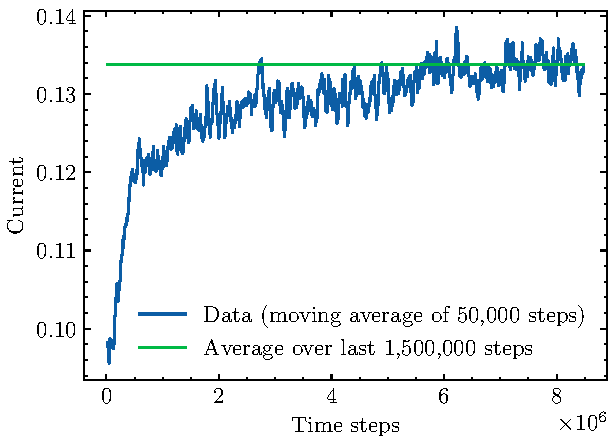
\includegraphics{speed_grad_current.pdf}
    \caption{Current as a function of the simulation time for the smarticle agent trained with the \texttt{speed\_gradient\_reward} function with $a=0.4$ and an almost uniform speed distribution with width $\sigma=5$. The green line shows the average current during the last 1.5 million time steps of the simulation, which is at about $0.134$, outperforming the last policy by about 15\% and the baseline by about 157\%.}
    \label{fig:speed_grad_current}
\end{figure}

After these results, it is clear that even if the lane strategy may not be \textit{the} most efficient transport strategy for the TASEP, it still clearly outperforms the meandering flow strategy and is therefore a very promising approach. The next step will be to try to encourage the formation of lanes in a more natural way, without explicitly supplying the smarticles with the desired structure.
\\
The current approach for the lane formation is not easy to implement in a real-world application, as it requires the smarticles to communicate in order to agree on a common origin. One could of course also think about the smarticles moving in an external potential, but this could hardly be called a \textit{physical} potential. It would have to be a trapping potential in one direction, while allowing movement in the other direction and most importantly, the minimum of the potential (the location of the trap) would have to be different for different speeds. Research on such potentials has been done in the context of trapped ion quantum computers, giving rise for example to the Paul trap \cite[II.A]{bruzewicz_trapped-ion_2019}. It would however be easier if the smarticles could form lanes just by local interactions. This is what we will try to achieve in the next section.

\subsection{Global Structures - The Nice Way}
% later binning speeds
% incorporate absolute speed into reward for different treatment
% agent naturally learns to follow the "forces", reward optimization is like energy minimization
In this second structure emergence experiment, we will try to let global structures emerge just from local \enquote{interactions}. Local interactions, in this context, are again the physical analogy to what we're really doing: Finding a reward function that is just based on the observation of a single particle. This, however, is a much harder endeavor than the previous approach. We will therefore introduce two modifications to the experiment:
\begin{enumerate}
    \item We will limit the speed distribution to a binary distribution, with only two speeds: $0.25$ and $0.95$. This will make it easier for the smarticles to form lanes, as it reduces the complexity of the problem. Instead of a quasi-continuous gradient, the smarticles now only have to form two distinct lanes.
    \item We will use two different neural networks (pairs of networks) for the two types of particles as explained in \ref{subsubsec:implementation-train}. Although the network was already supplied the speed of the current particle as an input feature, it is still much easier this way. When two types of particles have to behave differently, it means that the same input vector has to be mapped to an entirely different output vector in some situations, just based on the speed of the particle. To facilitate this, we would want the network weights to depend on the speed of the current particle, which is what we achieve by using two different networks. Furthermore, the performance the simulation is hardly affected by this change, as only one of the networks has to be used at any given time step. Training does, however, take twice as long, as each network only receives half the training data (only the transitions of the particles with the corresponding speed).
\end{enumerate}
The hardest part of this experiment is to find a suitable reward function. I will just present a working reward function here, before we proceed to analyze it. The reward function that is used in the smarticles package to achieve the emergence of lanes is defined as follows:
\begin{equation}
    \text{V}(r, \Delta v) = \begin{cases}
        -0.125 \cdot r + 0.625 & \text{if } \Delta v < 0.5 \text{ and } 1.5 < r \le 5 \\
        -0.75 \cdot r^{-1.3} - 0.15 & \text{if } \Delta v \ge 0.5 \text{ and } r \le 3.5 \\
        0 & \text{otherwise} \text{,}
    \end{cases}
\end{equation}
where $r$ is the distance between two particles and $\Delta v$ is the difference in speed between them. This pairwise potential is taken between the current particle and every other particle in its observation and summed up to form the reward. 
\\
\\
This might look complicated at first, but it will make sense after analyzing its basic properties. Let's turn to figure \ref{fig:lane_reward_func_3d} to get a better understanding of the reward function. We start by looking at the portion of the potential for $\Delta v > 0.5$ (the front left part of the plot). Here, the potential is less than or equal to zero for all distances. For distances larger than $r=3.5$, the potential is zero. For smaller distances, the potential is negative and decreases with decreasing distance. This just means that the agent is punished (negative reward) for being close to particles that have a very different speed ($\Delta v > 0.5$). This part tries to separate the fast and slow particles, but it isn't enough to form lanes already. Imagine a crowd of two kinds of people, homogeneously mixed. If everyone just tries to keep their distance to people of the other kind, the result will still be a mixed crowd with no structure.
\\
This is where the posterior portion of the potential comes into play. For $\Delta v < 0.5$, the potential is positive and increases with decreasing distance. This means that the agent is rewarded for being close to particles with a similar speed. For distances smaller than $r=1.5$, the potential drops back to zero, so as to keep the density inside the lanes low enough to move.
\\
\\
The combination of these two potentials is what makes the lanes emerge. The particles are rewarded for clustering together with particles of similar speed and these clusters are then separated by the negative reward between particles of different speeds. If the reward for forward moves is high enough compared to the clustering reward, the clusters will naturally stretch out in the forward direction, forming lanes.

\begin{figure}[H]
    \centering
    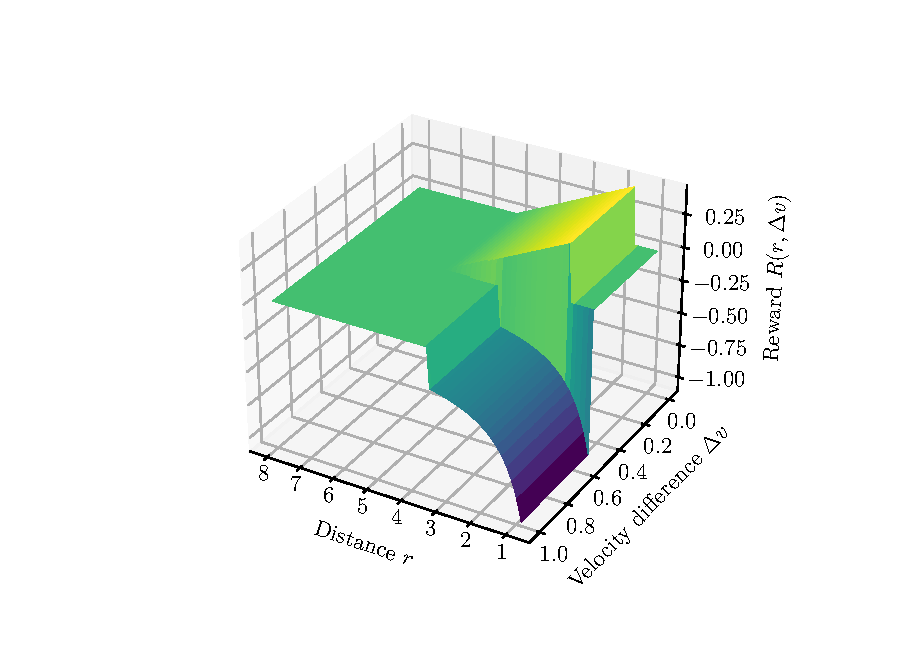
\includegraphics{lane_reward_func_3d_cropped.pdf}
    \caption{The reward function (\enquote{potential}) that achieves the emergence of large fast and slow lanes in the system. It takes the velocity difference and the distance between two particles as input. The potential is calculated between the agent and every other particle in the current observation and then summed up.}
    \label{fig:lane_reward_func_3d}
\end{figure}

After calling this function \enquote{potential} for the last few paragraphs, let's quickly look at why this makes sense. A physical potential gives rise to a force (its gradient) which drives the particles toward a configuration of (locally) minimal energy. In our case, the total reward takes the role of the energy and the algorithm tries to \textit{maximize} it. This is why contrary to physics, the negative areas of our potential are repulsive, while the positive areas are attractive. The \enquote{forces} in our case are encoded into the learned policy of the smarticles. In the general case of a partly stochastic policy, one could call these forces \enquote{voluntary forces}, as an agent doesn't necessarily follow the force that is applied to it. Another important distinction is that when the discount factor is large enough, the agent will value the future reward higher than the immediate reward. This can lead to a policy that actually moves away from a local maximum of the reward, if it can reach a higher maximum in the future. This is something that fundamentally distinguishes smart matter from physical matter, as physical matter will always move towards a local minimum of the potential, possibly getting stuck in a local minimum that is not the global minimum. (Note that this \textit{can} of course also happen in smart matter)
\\
\\
The proposed reward structure was put to the test in different trainings and subsequent simulations. Training an agent with a complicated reward function makes the training process less stable, and the final policies may differ. Depending on which exact realization of the lanes is discovered first, policies can have a slight bias towards a lane tilt in either direction or a suboptimal tendency to cluster also in the horizontal direction, leading to jams. I will present different approaches to mitigate these problems in the future, after the analysis of the current performance. Figure \ref{fig:lanes} shows two screenshots of different trained agents. While policy in figure \ref{fig:lanes_straight} has learned to form straight, horizontal lanes, the policy in figure \ref{fig:lanes_tilt} has a slight bias towards going up, leading to a tilted lane structure. Furthermore, both screenshots show a two to three cell gap between the lanes. This is suboptimal, as the unused space could be filled with particles, lowering the mean density in the lanes and therefore increasing the current. 

\begin{figure}[H]
    \centering
    \begin{subfigure}{\textwidth}
        \centering
        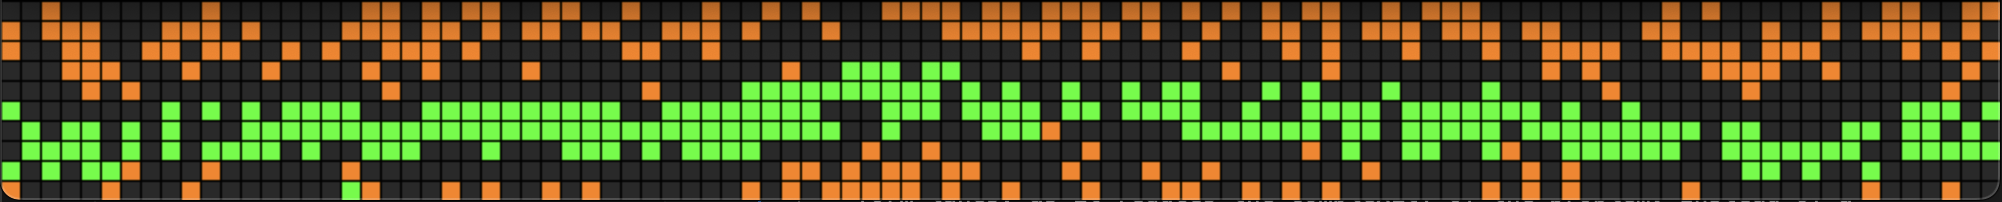
\includegraphics[width=\textwidth]{lanes_straight.png}
        \caption{These agents have learned to form straight lanes}
        \label{fig:lanes_straight}
    \end{subfigure}
    \vskip\baselineskip
    \begin{subfigure}{\textwidth}
        \centering
        
\includegraphics[width=\textwidth]{lanes_tilt.png}
        \caption{These agents have learned a small bias towards going up, leading to a tilted lane structure}
        \label{fig:lanes_tilt}
    \end{subfigure}
    \caption{Screenshots of the real-time visualizations of the simulation for two different policies trained with the \texttt{lane\_reward} function. The agents have learned to form lanes, but the lanes are not always perfectly straight. The environment has a density of $\rho=0.4$ and a binary speed distribution with speeds $0.25$ and $0.95$.}
    \label{fig:lanes}
\end{figure}

\begin{figure}[h]
    \centering
    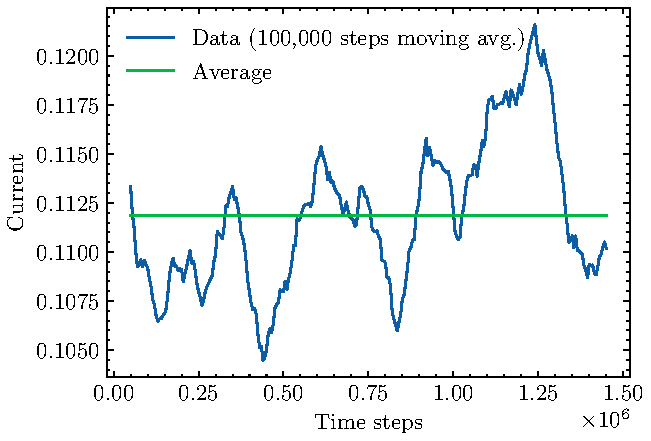
\includegraphics{lanes_current.pdf}
    \caption{Current as a function of the simulation time for the smarticle agent trained with the \texttt{lane\_reward} function. The green line shows the average current, which is at about $0.112$. The current is consistently higher than the baseline, but lower than that of the previous policies.}
    \label{fig:lanes_current}
\end{figure}

For one of the lane-forming agents, the current was again measured over time. The results are shown in figure \ref{fig:lanes_current}. The current fluctuates around a mean value of about $0.112$. We don't have a baseline for this configuration yet, as the density has been changed to $\rho=0.4$ to make the organization easier and mean speed is now $0.6$, which is higher than the speed of the baseline. We can set an optimistic baseline using equation \ref{eq:current_theory}, yielding $J_{\text{baseline}}=0.4\cdot(1-0.4)\cdot0.6\cdot0.5=0.072$. The current of the lane-forming policy would then be about 56\% higher than the baseline, but a lot lower than the current of the previous policies. The magnitude of the fluctuations is about $0.02$, about as large as that of the meandering flow policy. The speed gradient policy has a much smaller fluctuation amplitude, as the \enquote{hard coded} structure of the lanes is much more stable than the emergent structure.
